% $Id: step1.tex 4605 2014-01-30 08:49:42Z kanschat $

%%%%%%%%%%%%%%%%%%%%%%%%%%%%%%%%%%%%%%%%%%%%%%%%%%%%%%%%%%%%%%%%%%%%%% 
%%%%%%%%%%%%%%%%%%%%%%%%%%%%%%%%%%%%%%%%%%%%%%%%%%%%%%%%%%%%%%%%%%%%%% 
\section[Mesh]{Creating and refining a mesh}
\frame{\tableofcontents[currentsection,hideothersubsections]}

%%%%%%%%%%%%%%%%%%%%%%%%%%%%%%%%%%%%%%%%%%%%%%%%%%%%%%%%%%%%%%%%%%%%%%
\begin{frame}
  \frametitle{Tutorial Step 1}
  {\footnotesize{\url{http://www.dealii.org/\dealrelease/doxygen/deal.II/step_1.html}}}
  \begin{itemize}
  \item Two examples of creating a mesh
    \begin{itemize}
    \item Polygonal domain
    \item Curved boundary
    \end{itemize}
  \item Two ways of refining a mesh
    \begin{itemize}
    \item globally/quasi-uniform
    \item locally
    \end{itemize}
  \end{itemize}
\end{frame}

%%%%%%%%%%%%%%%%%%%%%%%%%%%%%%%%%%%%%%%%%%%%%%%%%%%%%%%%%%%%%%%%%%%%%%
\subsection{Header files}
\begin{frame}
  \frametitle{The tedious header files}
  \begin{block}{}
  \lstinputlisting{tutcode/step1-1.cc}    
  \end{block}
\end{frame}

%%%%%%%%%%%%%%%%%%%%%%%%%%%%%%%%%%%%%%%%%%%%%%%%%%%%%%%%%%%%%%%%%%%%%%
\subsection{Mesh generation}
\begin{frame}
  \frametitle{A regular square mesh}
  \begin{block}{}
    \lstinputlisting{tutcode/step1-2.cc}    
  \end{block}

  \begin{itemize}
  \item \lstinline!Triangulation<2>! is a two-dimensional mesh
  \item \lstinline!GridGenerator! functions create a mesh
  \item \lstinline!GridOut! writes a mesh as a graphics file
  \end{itemize}
\end{frame}

%%%%%%%%%%%%%%%%%%%%%%%%%%%%%%%%%%%%%%%%%%%%%%%%%%%%%%%%%%%%%%%%%%%%%%
\begin{frame}
  \frametitle{Syntax conventions}
  \begin{itemize}
  \item Classes in dealii
    \begin{itemize}
    \item CamelCase
    \item \lstinline!GridOut!, \lstinline!Triangulation<2>!
    \end{itemize}
  \item Functions, variables
    \begin{itemize}
    \item Lower case, words separated by underscore
    \item \lstinline!triangulation!, \lstinline!refine_global!,
      \lstinline!GridGenerator::hyper_cube!
    \end{itemize}
  \item Namespaces in dealii
    \begin{itemize}
    \item Inconsistent
    \item \lstinline!GridGenerator!
    \end{itemize}
  \end{itemize}
\end{frame}

%%%%%%%%%%%%%%%%%%%%%%%%%%%%%%%%%%%%%%%%%%%%%%%%%%%%%%%%%%%%%%%%%%%%%%
\begin{frame}
  \frametitle{A regular square mesh}
  \begin{center}
    
\includegraphics[height=.8\textheight]{graph/step1-1}
  \end{center}
\end{frame}

%%%%%%%%%%%%%%%%%%%%%%%%%%%%%%%%%%%%%%%%%%%%%%%%%%%%%%%%%%%%%%%%%%%%%%
\begin{frame}
  \frametitle{The mesh hierarchy}
  \begin{center}
    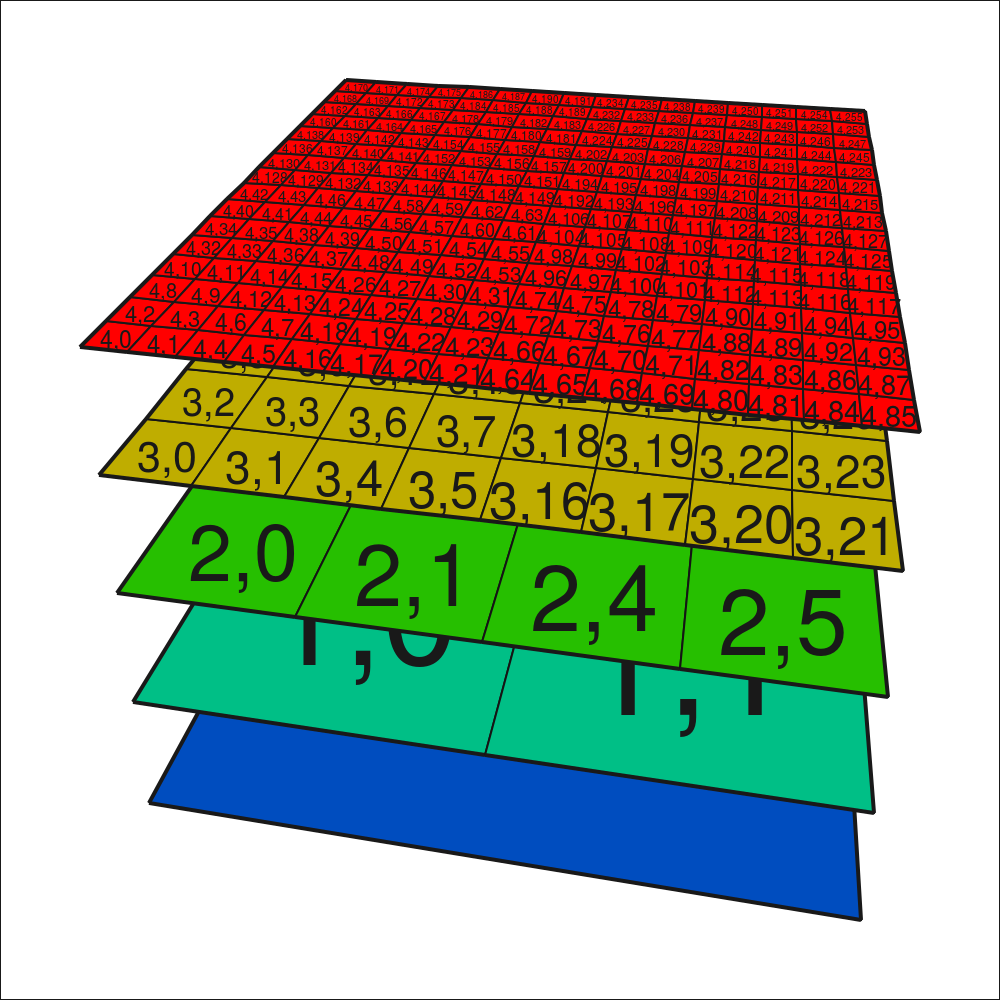
\includegraphics[height=.9\textheight]{graph/step1-1a}
  \end{center}
\end{frame}

%%%%%%%%%%%%%%%%%%%%%%%%%%%%%%%%%%%%%%%%%%%%%%%%%%%%%%%%%%%%%%%%%%%%%%
\begin{frame}
  \frametitle{Mesh facts}
  \begin{itemize}
  \item \lstinline!Triangulation<dim>! always stores a hierarchy of
    mesh levels.
  \item A cell is identified by its level and an index inside the level
  \item The level of a cell is its distance by refinement from the
    original mesh
  \item Levels are modeled like STL containers
  \begin{block}{Loop over all cells of a level}
    \lstinputlisting[basicstyle=\footnotesize]{tutcode/step1-3a.cc}  
  \end{block}
  \end{itemize}
\end{frame}

\subsection{Local refinement}
%%%%%%%%%%%%%%%%%%%%%%%%%%%%%%%%%%%%%%%%%%%%%%%%%%%%%%%%%%%%%%%%%%%%%%
\begin{frame}
  \frametitle{Local refinement}
  \begin{columns}
    \begin{column}{.5\textwidth}
      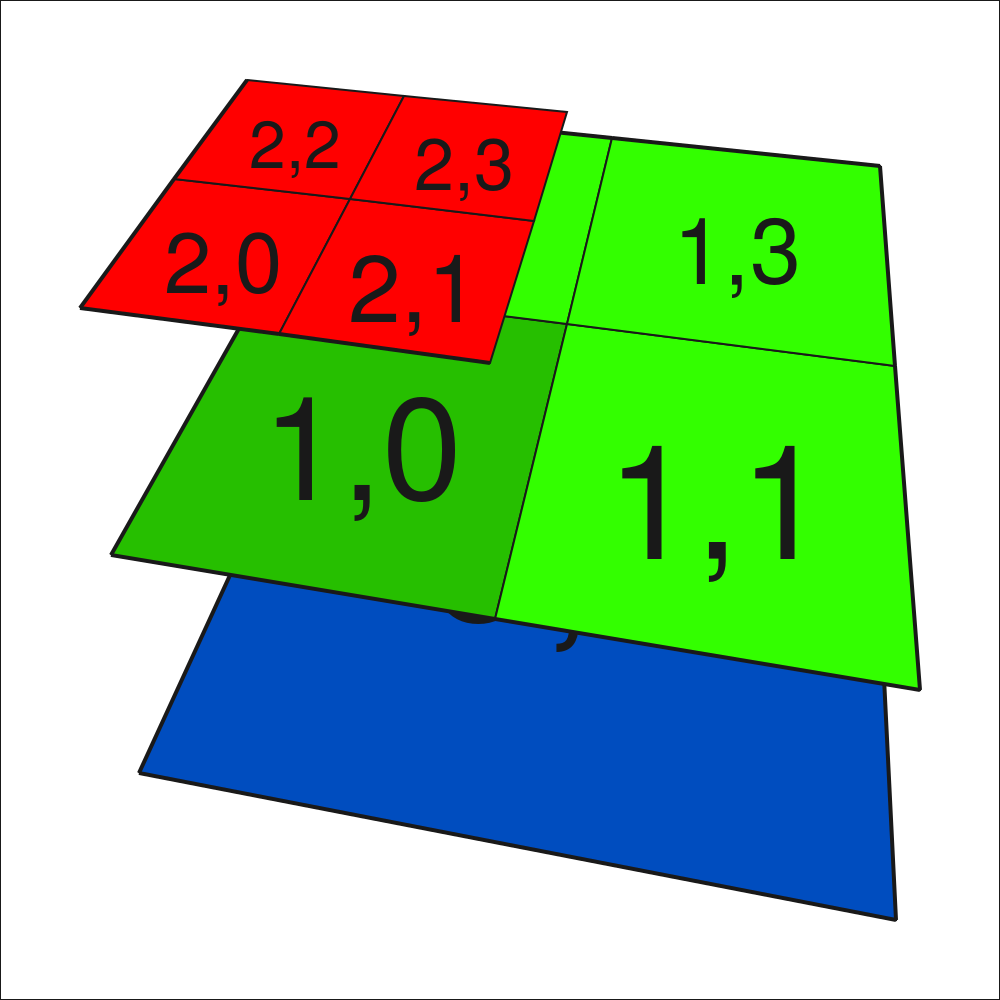
\includegraphics[width=\textwidth]{graph/step1-1b}
    \end{column}
    \begin{column}{.5\textwidth}
      \begin{itemize}
      \item Meshes can be refined to different levels in different regions
      \item Cells are still defined by level and index
      \end{itemize}
    \end{column}
  \end{columns}
\end{frame}

%%%%%%%%%%%%%%%%%%%%%%%%%%%%%%%%%%%%%%%%%%%%%%%%%%%%%%%%%%%%%%%%%%%%%%
\begin{frame}
  \frametitle{Locally refined mesh}
  \begin{columns}
    \begin{column}{.4\textwidth}
      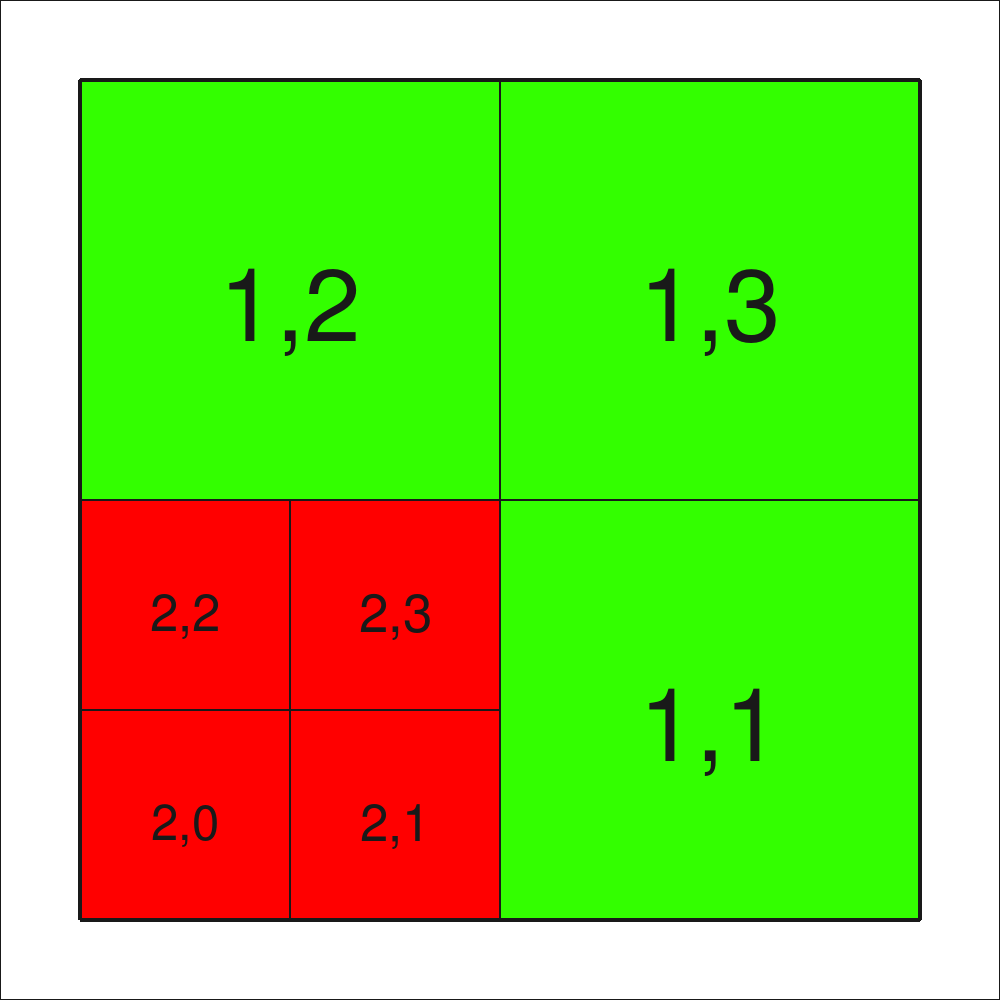
\includegraphics[width=\textwidth]{graph/step1-1c}
    \end{column}
    \begin{column}{.6\textwidth}
      \begin{itemize}
      \item Cells belong to different levels
        \item Cells visible in this graph are called active
          \begin{itemize}
          \item They are the leaves of the refinement tree
          \item They are the actual mesh for computation
          \end{itemize}
      \item We need a new iterator
      \end{itemize}
    \end{column}
  \end{columns}
  \pause
  \begin{block}{Loop over all active cells}
    \lstinputlisting[basicstyle=\footnotesize]{tutcode/step1-3b.cc}  
  \end{block}
\end{frame}

%%%%%%%%%%%%%%%%%%%%%%%%%%%%%%%%%%%%%%%%%%%%%%%%%%%%%%%%%%%%%%%%%%%%%%
\begin{frame}
  \frametitle{The second mesh}
  \begin{center}
    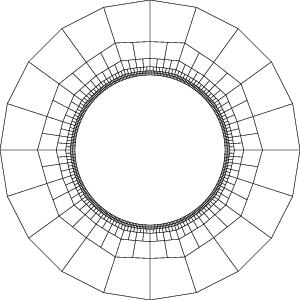
\includegraphics[height=.8\textheight]{graph/step1-2}
  \end{center}  
\end{frame}

%%%%%%%%%%%%%%%%%%%%%%%%%%%%%%%%%%%%%%%%%%%%%%%%%%%%%%%%%%%%%%%%%%%%%%
\begin{frame}
  \frametitle{Setting up the curved geometry}
  \begin{block}{}
    \lstinputlisting[basicstyle=\footnotesize]{tutcode/step1-3.cc}
  \end{block}
\end{frame}

%%%%%%%%%%%%%%%%%%%%%%%%%%%%%%%%%%%%%%%%%%%%%%%%%%%%%%%%%%%%%%%%%%%%%%
\begin{frame}
  \frametitle{Local refinement: cell loops}
  \begin{block}{}
    \lstinputlisting{tutcode/step1-4.cc}    
  \end{block}

  \begin{itemize}
  \item Run through all \textit{active} cells of the mesh
    \begin{itemize}
    \item Use iterators like pointers into an array (STL)
    \item Ingore coarse cells in the refinement hierarchy
    \end{itemize}
  \end{itemize}
\end{frame}

%%%%%%%%%%%%%%%%%%%%%%%%%%%%%%%%%%%%%%%%%%%%%%%%%%%%%%%%%%%%%%%%%%%%%%
\begin{frame}
  \frametitle{Local refinement: select cells}
  \begin{block}{}
    \lstinputlisting[basicstyle=\footnotesize]{tutcode/step1-5.cc}    
  \end{block}
  
  \begin{itemize}
  \item Marke all cells with a vertex on the inner perimeter
  \end{itemize}
\end{frame}

%%%%%%%%%%%%%%%%%%%%%%%%%%%%%%%%%%%%%%%%%%%%%%%%%%%%%%%%%%%%%%%%%%%%%%
\begin{frame}
  \frametitle{Local refinement: the refinement loop}
  \begin{block}{}
    \lstinputlisting[basicstyle=\footnotesize]{tutcode/step1-6.cc}    
  \end{block}

  \begin{itemize}
  \item Create five levels of local refinement
  \end{itemize}
\end{frame}

%%%%%%%%%%%%%%%%%%%%%%%%%%%%%%%%%%%%%%%%%%%%%%%%%%%%%%%%%%%%%%%%%%%%%%
\begin{frame}
  \frametitle{Local refinement: the whole function}
  \footnotesize\lstinputlisting[basicstyle=\tiny]{tutcode/step1-7.cc}
\end{frame}

%%%%%%%%%%%%%%%%%%%%%%%%%%%%%%%%%%%%%%%%%%%%%%%%%%%%%%%%%%%%%%%%%%%%%%
\begin{frame}
  \frametitle{The second mesh}
  \begin{center}
    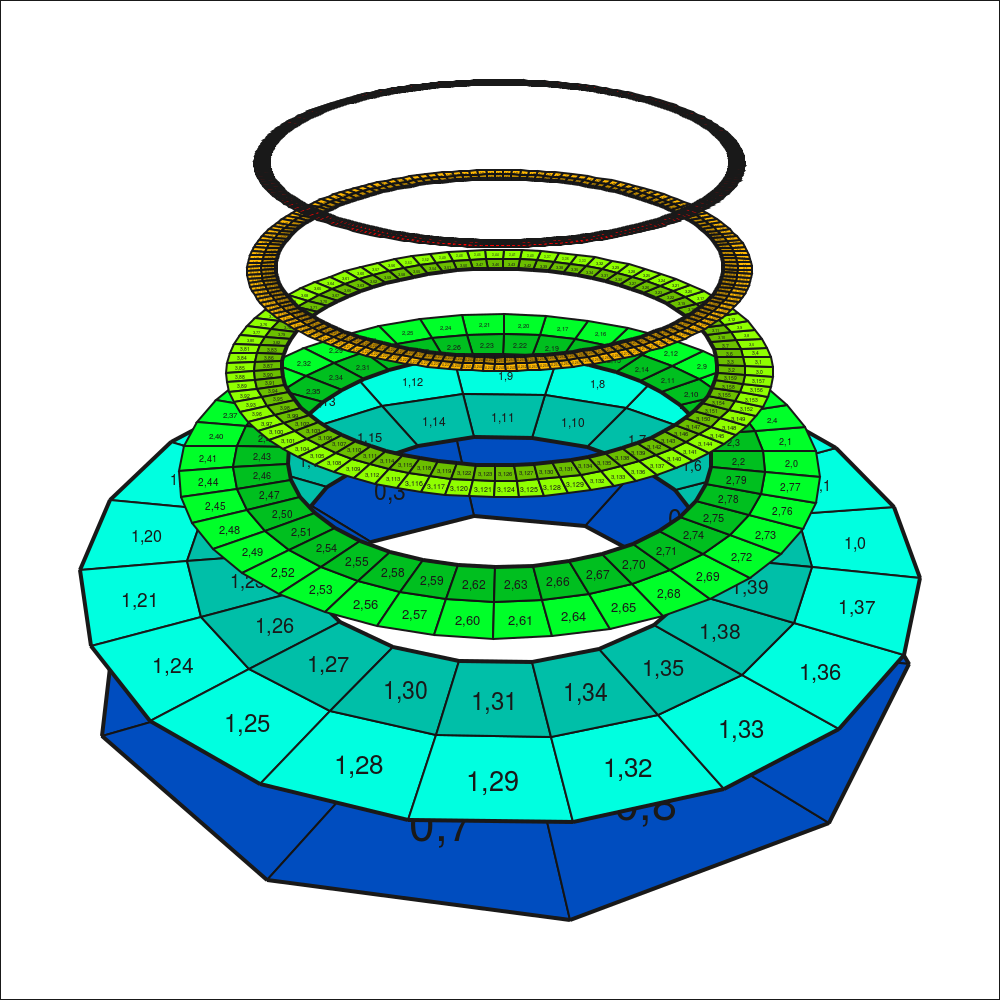
\includegraphics[height=.8\textheight]{graph/step1-2a}
  \end{center}  
\end{frame}

%%%%%%%%%%%%%%%%%%%%%%%%%%%%%%%%%%%%%%%%%%%%%%%%%%%%%%%%%%%%%%%%%%%%%%
\subsection{Problems}
\begin{frame}
  \frametitle{Step 1 Problems: meshes}
  \begin{enumerate}
    \item Locally refined square mesh
    \begin{enumerate}
    \item Create a mesh for the square $[-1,1]^2$ and refine once globally.
    \item On a given mesh refine all cells with at least one vertex in
      the cicle of radius $1/8$ around the origin. Repeat 6 times to
      resolve the circle.
    \item Visualize the result (gnuplot, SVG, or VTK). Use the online
      documentation to find options. Play!
    \end{enumerate}
  \item Generate a half open shell. How do inner and outer radius
    affect the shape of cells? Visualize!
  \end{enumerate}
\end{frame}

%%% Local Variables: 
%%% mode: latex
%%% TeX-master: "slides"
%%% End: 
